\subsection{Affine Varieties}


\begin{exercise}{2}
In $\R^2$, sketch $\bV(y^2-x(x-1)(x-2))$. Hint: For which $x$'s is it possible to solve for $y$? How many $y$'s correspond to each $x$? What symmetry does the curve have?
\end{exercise}
\begin{proof}
I will use a graphing calculator for this exercise, but still will answer the hint questions. If we solve for $y$, we obtain $y=\sqrt{x(x-1)(x-2)}$, so that we can solve for $y$, whenever $x(x-1)(x-2)\geq 0$. We require that either all of $x, x-1$ and $x-2$ are non-negative, or exactly two of them are negative. All of them are non-negative whenever $x\geq 2$ and two of them are negative whenever $0<x<1$. For these values of $x$ we have two values of $y$ (positive and negative), and hence we obtain symmetry with respect to the $x$-axis.
 \begin{figure}[H]
     \centering
     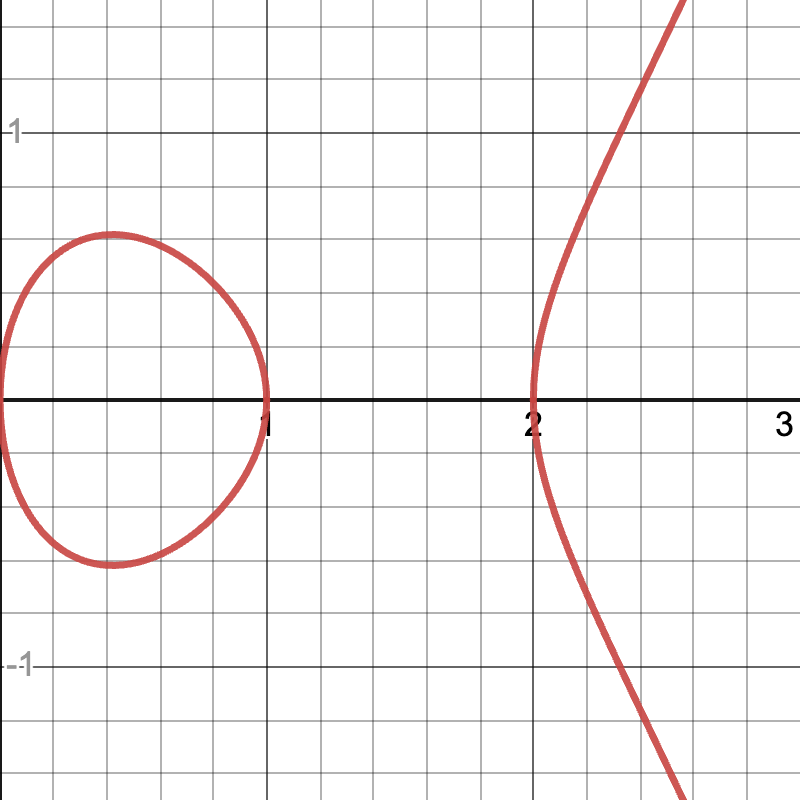
\includegraphics[width=.5\textwidth]{cox-little-oshea/assets/sec1-2-ex2.png}
     \caption{Graph of $\bV(y^2-x(x-1)(x-2))$}
     \label{fig:sec1-2-ex2}
 \end{figure}
\end{proof}

\begin{exercise}{3}
In the plane $\R^2$, draw a picture to illustrate $\bV(x^2+y^2-4)\cap\bV(xy-1)=\bV(x^2+y^2-4,xy-1)$, and determine the points of intersection. Note that this is a special case of lemma 2.
\end{exercise}
\begin{proof}
 \begin{figure}[H]
     \centering
     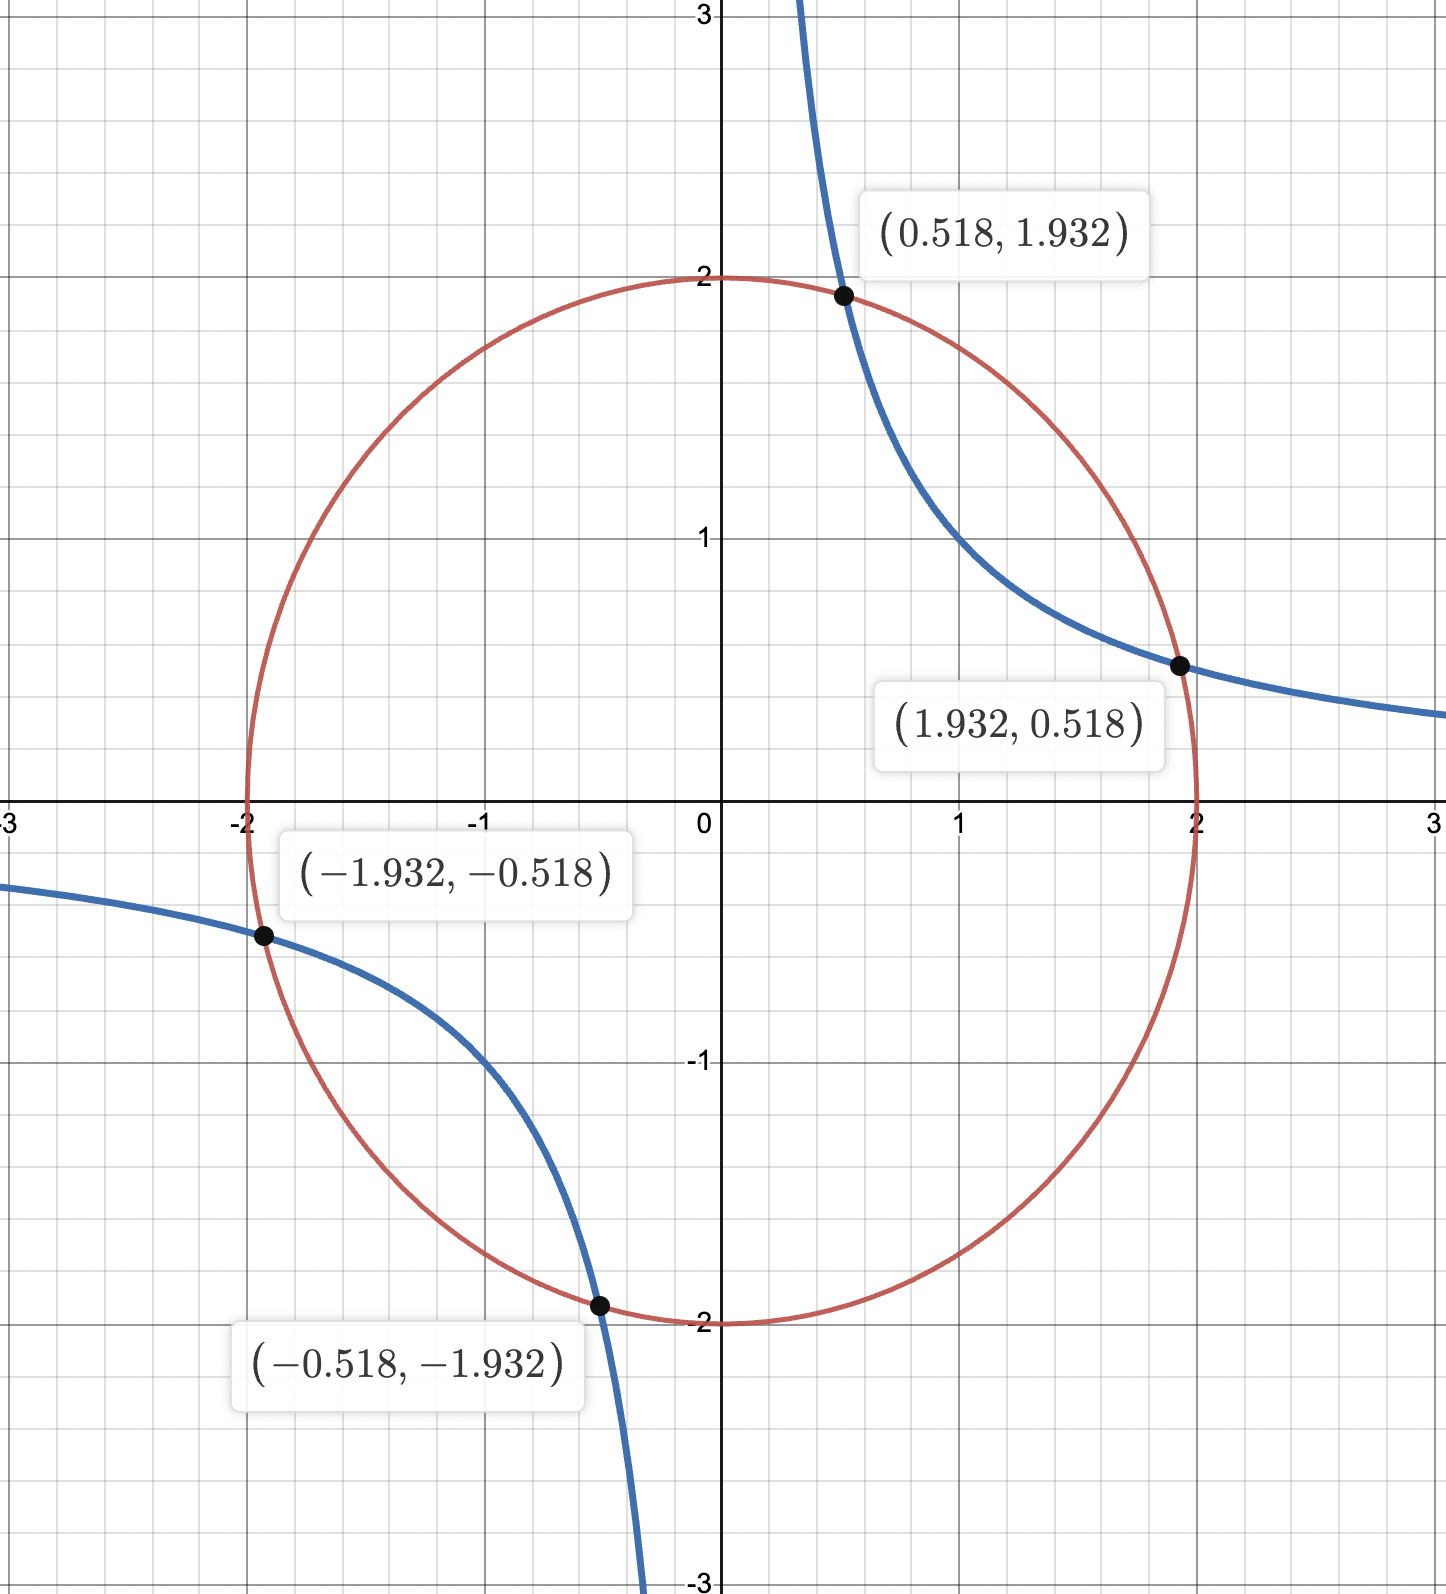
\includegraphics[width=.5\textwidth]{cox-little-oshea/assets/sec1-2-ex3.png}
     \caption{Graph of $\bV(x^2+y^2-4), \bV(xy-1)$, and its intersection points}
     \label{fig:sec1-2-ex3}
 \end{figure}
\end{proof}

\begin{exercise}{6}
Let us show that all finite subsets of $k^n$ are affine varieties.

\begin{enumerate}
    \item Prove that a single point $(a_1,\dots,a_n)\in k^n$ is an affine variety.
    \item Prove that every finite subset of $k^n$ is an affine variety. Hint: Lemma 2 will be useful.
\end{enumerate}
\end{exercise}
\begin{proof}
 \begin{enumerate}
     \item Consider the set of polynomials $f_1,\dots,f_n$ given by $f_i(x_i)=x_i-a_i$. Then certainly $\bV(f_1,\dots,f_n)$ has as variety the point $(a_1,\dots,a_n)\in k^n$, as required.
     \item We have just proven above that any point is an affine variety of a particular set of polynomials, so that for any point in the set we are interested in, say $(a_{i,1},\dots,a_{i,n})$ is a variety $\bV_i$ of a set of polynomials. From Lemma 2, we know that the union of two varieties is a variety, hence, $\cup_{i=1}^{m}\bV_i$ is a variety.
 \end{enumerate}
\end{proof}

\begin{exercise}{8}
It can take some work to show that something is not an affine variety. For example, consider the set $X=\{(x,x)\mid x\in\R, x\neq 1\}\subseteq\R^2$, which is the straight line $x=y$ with the point $(1,1)$ removed. To show that $X$ is not an affine variety, suppose that $X=\bV(f_1,\dots,f_s)$. Then each $f_i$ vanishes on $X$, and if we can show that $f_i$ also vanishes at $(1,1)$, we will get the desired contradiction. Thus, here is what you are to prove: if $f\in\R[x,y]$ vanishes on $X$, then $f(1,1)=0$. Hint: let $g(t)=f(t,t)$, which is a polynomial $\R[t]$. Now apply the proof of Proposition 5 of Section 1.
\end{exercise}
\begin{proof}
 If $f_i$ vanishes on $X$, then $f_i$ has infinitely many roots. But we know that a polynomial with infinitely many roots must be the zero polynomial. Hence, $f_i=0$ and $f_i(1,1)=0$, as required.
\end{proof}

\begin{exercise}{11}
So far we have discussed varieties of $\R$ or $\C$. It is also possible to consider varieties over the field $\Q$, although the questions here tend to be much harder. For example, let $n$ be a positive integer, and consider the variety $F_n\subseteq\Q^2$ defined by $x^n+y^n=1$. Notice that there are some obvious solutions when $x$ or $y$ is zero. We call these trivial solutions. An interesting question is whether or not there are nontrivial solutions.
\begin{enumerate}
    \item Show that $F_n$ has two trivial solutions if $n$ is odd and four trivial solutions if $n$ is even.
    \item Show that $F_n$ has a nontrivial solution for some $n\geq 3$ if and only if Fermat's Last Theorem were false.
\end{enumerate}
Fermat's Last Theorem states that, for $n\geq 3$, the equation $x^n+y^n=z^n$ has no solutions where $x,y$ and $z$ are nonzero integers. The general case of this conjecture was proved by Andrew Wiles in 1994 using some very sophisticated number theory. The proof is extremely difficult.
\end{exercise}
\begin{proof}
    \begin{enumerate}
        \item Odd $n$. The trivial solutions are characterised by $x=0$ or $y=0$. Without loss of generality, suppose $x=0$. Since $n$ is odd, if $y=-1$, then $y^n=-1$ so that the equation is not satisfied. Hence $y$ must be equal to 1. We can conclude the same for $x$ if $y=0$. So that there are 2 trivial solutions in total.

        Even $n$. We can follow the same approach as above. Simply notice that if $x=0$ and $y=-1$, we have that $y^n=1$ so that  $y=\pm1$ are valid solutions. We can reason the same for $x$ when $y=0$ so that we obtain 4 trivial solutions.
        \item ($\Rightarrow$) Suppose $F_n$ has a nontrivial solution. Then there exist $x/p,y/q\in\Q$ and $x,p,y,q\in\Z$ such that $(x/p)^n+(y/q)^n=1$. Let $k=\lcm(p,q)$, so that $k\in\Z$. Then $(xq)^n+(yp)^n=k^n$. Since $n\geq 3$ and $xq,yp,k\in\Z$ the equation from the previous sentence would imply that Fermat's Last Theorem is false.

        ($\Leftarrow$) Suppose Fermat's Last Theorem is false. Then there exist $x,y,z\in\Z$ such that $x^n+y^n=z^n$ for some $n\geq 3$. However, this implies $(x/z)^n+(y/z)^n=1$. That is, $p^n+q^n=1$, where $p,q\in\Q$, as required.
    \end{enumerate}
\end{proof}

\begin{exercise}{15}
In Lemma 2, we showed that if $V$ and $W$ are affine varieties, the so are their union $V\cup W$ and intersection $V\cap W$. In this exercise we will study how other set-theoretic operations affect affine varieties.
\begin{enumerate}
    \item Prove that finite unions and intersections of affine varieties are again affine varieties. Hint: Induction.
    \item Give an example to show that an infinite union of affine varieties need not be an affine variety. Hint: By exercises 8-10, we know some subset of $k^n$ that are not affine varieties. Surprisingly, an infinite intersection of affine varieties is still an affine variety. This is a consequence of the Hilbert Basis Theorem, which will be discussed in Chapters 2 and 4.
    \item Given an example to show that the set-theoretic difference $V\setminus W$ of two affine varieties need not be an affine variety.
    \item Let $V\subseteq k^n$ and $W\subseteq k^m$ be two affine varieties, and let $V\times W=\{(x_1,\dots,x_n,y_1,\dots,y_m)\in k^{n+m}\mid(x_1,\dots,x_n)\in V,(y_1,\dots,y_m)\in W\}$ be their Cartesian product. Prove that $V\times W$ is an affine variety in $k^{n+m}$. Hint: If $V$ is defined by $f_1,\dots,f_s\in k[x_1,\dots,x_n]$, then we can regard $f_1,\dots,f_s$ as polynomials in $k[x_1,\dots,x_n,y_1,\dots,y_m]$, and similarly for $W$. Show that this gives defining equations for the Cartesian product.
\end{enumerate}
\end{exercise}
\begin{proof}
    \begin{enumerate}
        \item We will prove by induction that finite unions of affine varieties are again affine varieties. The result for intersections can be proved in a similar manner. 

        Base case: the result in Lemma 2. Now suppose the result holds for the union of $n-1$ affine varieties, so that $\cap_{i=1}^{n-1}\bV_i$ is an affine variety. From Lemma 2, we know that $\cap_{i=1}^{n-1}\bV_i= \\\bV= {\set{f_1^1,\dots f_{s_1}^1,f_1^2,\dots,f_{s_2}^2,\dots,f_1^{n-1},\dots,f_{s_{n-1}}^{n-1}}}$, where $f_i^j$ corresponds to the $i$-th polynomial of the $j$-th affine variety. Certainly, $\cap_{i=1}^{n-1}\bV_i\cap \bV_n$ is an affine variety where $\cap_{i=1}^{n-1}\bV_i\cap \bV_n= \bV=\set{f_1^1,\dots,f_{s_{n-1}}^{n-1},f_1^n,\dots,f_{s_n}^n}$, as required.
        \item In Exercise 6, we proved that any single point in $k^n$ is an affine variety. Consider the infinite union of single points $(x,x)$ where $x\in\R\setminus\set{1}$. Then we obtain the set $X=\set{(x,x)\mid x\in\R,x\neq 1}$, which we proved in exercise 8, is not an affine variety.
        \item Consider the affine variety given by $X'=\set{(x,x)\mid x\in\R}$ and the set $\set{(1,1)}$. We have $X=X'\setminus\set{(1,1)}$, which we proved is not an affine variety.
        \item Following the hint, we consider $f_1,\dots,f_s,g_1,\dots,g_t\in k[x_1,\dots,x_n,y_1,\dots,y_m]$. We then have that for any $(x_1,\dots,y_m)\in V\times W$, and any $h_i\in\\ \set{f_1,\dots,f_s,g_1,\dots,g_t}$, $h_i(x_1,\dots,y_m)=0$, given that, if $h_i=f_j$ for some $j$, then $f_j(x_1,\dots,y_m)=0$ by virtue of $(x_1,\dots,x_n)\in V$ and likewise for $h_i=g_j$. Then, $V\times W$ is an affine variety, where the defining polynomials are $\set{f_1,\dots,f_s,g_1,\dots,g_t}\in k[x_1,\dots,x_n,y_1,\dots,y_m]$, as required.
    \end{enumerate}
\end{proof}
